\documentclass[a4paper]{article}
\usepackage[T1]{fontenc}			% pacchetto per \chapter
\usepackage[italian]{babel}
\usepackage[italian]{isodate}  		% formato delle date in italiano
\usepackage{graphicx}				% gestione delle immagini
\usepackage{amsfonts}
\usepackage{booktabs}				% tabelle di qualità superiore
\usepackage{mathrsfs, amsmath}				% pacchetto matematica
\usepackage{mathtools}				% per sottolineare sotto le equazioni
\usepackage{stmaryrd} 				% per '\llbracket' e '\rrbracket'
\usepackage{amsthm}					% teoremi migliorati
\usepackage{enumitem}				% gestione delle liste
\usepackage{pifont}					% pacchetto con elenchi carini
\usepackage{enumitem}				% pacchetto per elenchi con lettere dell'alfabeto
\usepackage{cancel}					% per cancellare delle espressioni matematiche
\usepackage{listings}				% implementa codice di programmazione
\usepackage{mathalpha}
\usepackage{caption}


\usepackage[x11names]{xcolor}		% pacchetto colori RGB
% Link ipertestuali per l'indice
\usepackage{xcolor}
\usepackage[linkcolor=black, citecolor=blue, urlcolor=cyan]{hyperref}
\hypersetup{
	colorlinks=true
}

% Colour code style
\definecolor{codegreen}{rgb}{0,0.6,0}
\definecolor{codegray}{rgb}{0.5,0.5,0.5}
\definecolor{codepurple}{rgb}{0.58,0,0.82}
\definecolor{backcolour}{rgb}{0.95,0.95,0.92}

\lstdefinestyle{MATLAB}{
	backgroundcolor=\color{backcolour},   
	commentstyle=\color{codegreen},
	keywordstyle=\color{magenta},
	numberstyle=\tiny\color{codegray},
	stringstyle=\color{codepurple},
	basicstyle=\ttfamily\footnotesize,
	breakatwhitespace=false,         
	breaklines=true,                 
	captionpos=b,                    
	keepspaces=true,                 
	numbers=left,                    
	numbersep=5pt,                  
	showspaces=false,                
	showstringspaces=false,
	showtabs=false,                  
	tabsize=2
}
\lstset{style=MATLAB}

%\usepackage{showframe}				% visualizzazione bordi
%\usepackage{showkeys}				% visualizzazione etichetta

\newtheorem{theorem}{\textcolor{Red3}{\underline{Teorema}}}
\newtheorem{lemma}{Lemma}
\renewcommand{\qedsymbol}{QED}
\newcommand{\exec}[1]{\llbracket #1\:\rrbracket}
\newcommand{\dquotes}[1]{``#1''}
\newcommand{\longline}{\noindent\rule{\textwidth}{0.4pt}}

\begin{document}
	\author{Università degli Studi di Verona}
	\title{Soluzione - Simulazione di Elaborazione di segnali e immagini}
	\date{{\Large 14 Giugno 2021}}
	\maketitle
	
	\section{Soluzione Esercizio (4 punti)}
	
	Prima di eseguire le operazioni è necessario comprendere che tipo di filtro è. Per farlo, si guarda la sua maschera, quindi la matrice, e si cerca di ricordare quale sia.\newline
	
	\noindent
	Si esclude a priori un filtro di \emph{smoothing} di tipo media e mediana poiché la prima ha i coefficienti tutti uguali, mentre la seconda non utilizza una maschera di questo tipo (semplicemente viene presa le mediana).\newline
	
	\noindent
	Ricordandosi anche i vari operatori per estrarre l'edge:
	\begin{itemize}
		\item Gradiente discreto:
		\begin{equation*}
			\dfrac{\partial f}{\partial x}\left[x,y\right] \approx F\left[x+1, y\right] - F\left[x,y\right]
		\end{equation*}
		
		\item Operatore di Roberts utilizza due tipi di maschere:
		\begin{equation*}
			S_{1} = \begin{bmatrix}
				1 & 0 \\
				0 & -1
			\end{bmatrix} \hspace{2em} S_{2} = \begin{bmatrix}
			0 & 1 \\
			-1 & 0
		\end{bmatrix}
		\end{equation*}
	
		\item Operatore di Prewitt con maschere del tipo:
		\begin{equation*}
			S_{x} = \begin{bmatrix}
				-1 & 0 & 1 \\
				-1 & 0 & 1 \\
				-1 & 0 & 1
			\end{bmatrix} \hspace{2em} S_{y} = \begin{bmatrix}
				1 & 1 & 1 \\
				0 & 0 & 0 \\
				-1 & -1 & -1
			\end{bmatrix}
		\end{equation*}
		
		\item Operatore di Sobel che ha varie maschere ma le più famose:
		\begin{equation*}
			S_{x} = \begin{bmatrix}
				-1 & 0 & 1 \\
				-2 & 0 & 2 \\
				-1 & 0 & 1
			\end{bmatrix} \hspace{2em} S_{y} = \begin{bmatrix}
				1 & 2 & 1 \\
				0 & 0 & 0 \\
				-1 & -2 & -1
			\end{bmatrix}
		\end{equation*}
	
		\item Operatore di Kirsch che ha ben 8 maschere direzionali, qui di seguito se ne riportano solo quattro:
		\begin{equation*}
			\begin{array}{lllc}
				\text{Horizontal line: } & D_{0} & = & \begin{bmatrix}
					-1 & -1  & -1 \\
					2 & 2 & 2 \\
					-1 & -1 & -1
				\end{bmatrix} \\
				&&& \\
				45\text{ line: } & D_{45} & = & \begin{bmatrix}
					-1 & -1  & 2 \\
					-1 & 2 & -1 \\
					2 & -1 & -1
				\end{bmatrix} \\
				&&& \\
				\text{Vertical line: } & D_{90} & = & \begin{bmatrix}
					-1 & 2  & -1 \\
					-1 & 2 & -1 \\
					-1 & 2 & -1
				\end{bmatrix} \\
				&&& \\
				135\text{ line: } & D_{135} & = & \begin{bmatrix}
					2 & -1  & -1 \\
					-1 & 2 & -1 \\
					-1 & -1 & 2
				\end{bmatrix} \\
			\end{array}
		\end{equation*}
	
		\item Operatore di Roberts che ha 8 maschere direzionali simili a quelle di Kirsch.
	\end{itemize}
	Si deduce che neanche l'estrazione dell'edge assomiglia al filtro proposto.\newline
	
	\noindent
	Dunque, andando ad approfondire i filtri di \emph{sharpening} si trovano due categorie: \emph{basic highpass spatial filtering} e \emph{high boost filtering}. Si conclude che il filtraggio scelto è il filtro \emph{\textbf{basic highpass spatial filtering}} che utilizza il \textbf{filtro laplaciano}. La scelta è stata determinata da due fattori:
	\begin{enumerate}
		\item Se fosse stato scelto un filtro \emph{high boost filtering}, sarebbe stata necessaria sia l'immagine prima dello \emph{smoothing}, sia l'immagine dopo aver applicato tale operazione. Questo perché, il filtro lavora eseguendo una differenza tra l'immagine filtrata e quella originale.
		
		\item Si ricorda la forma generale della maschera del filtro laplaciano:
		\begin{equation*}
			h = \dfrac{1}{\alpha + 1} \begin{bmatrix}
				-\alpha & \alpha-1 & -\alpha \\
				\alpha-1 & \alpha+5 & \alpha-1 \\
				-\alpha & \alpha-1 & -\alpha
			\end{bmatrix}
		\end{equation*}
		E si ricorda anche una tipica maschera di filtraggio laplaciana utilizzata dal filtro \emph{basic highpass spatial filtering}:
		\begin{equation*}
			\dfrac{1}{9} \times \begin{bmatrix}
				0 & -1 & 0 \\
				-1 & 4 & -1 \\
				0 & -1 & 0
			\end{bmatrix}
		\end{equation*}
	\end{enumerate}\newpage
	
	\noindent
	Adesso si eseguono le operazioni di filtraggio usando il laplaciano. I passaggi sono: si va nelle coordinate richieste, per esempio $\left(2,2\right)$; si estrae una matrice grande quanto il filtro e contenente i valori vicini alla coordinata, quindi in questo caso si estrae una matrice $3 \times 3$ centrata in $\left(2,2\right)$; si moltiplica la matrice estratta con il filtro; si esegue una differenza tra il valore centrale della matrice e i valori circostanti; si moltiplica il risultato per l'eventuale frazione; infine si sostituiscono i valori nella matrice originaria.\newline
	
	\noindent
	Si estraggono le matrici dall'immagine originale e si moltiplica per la maschera:
	\begin{equation*}
		\begin{array}{lllll}
			\left(2,2\right) & \xrightarrow{\text{estrazione}} & \begin{bmatrix}
				200 & 200 & 200 \\
				200 & 200 & 200 \\
				200 & 200 &  50
			\end{bmatrix} \cdot \begin{bmatrix}
				0 & -1 & 0 \\
				-1 & 8 & -1 \\
				0 & -1 & 0
			\end{bmatrix} & = & \begin{bmatrix}
				0 & -200 & 0 \\
				-200 & 1600 & -200 \\
				0 & -200 & 0
			\end{bmatrix} \\
			%
			\\
			%
			\left(3,3\right) & \xrightarrow{\text{estrazione}} & \begin{bmatrix}
				200 & 200 & 200 \\
				200 &  50 &  50 \\
				200 &  50 &  50
			\end{bmatrix} \cdot \begin{bmatrix}
				0 & -1 & 0 \\
				-1 & 8 & -1 \\
				0 & -1 & 0
			\end{bmatrix} & = & \begin{bmatrix}
				0 & -200 & 0 \\
				-200 & 400 & -50 \\
				0 & -50 & 0
			\end{bmatrix} \\
			%
			\\
			%
			\left(4,4\right) & \xrightarrow{\text{estrazione}} & \begin{bmatrix}
				50 & 50 & 50 \\
				50 & 50 & 50 \\
				50 & 50 & 50
			\end{bmatrix} \cdot \begin{bmatrix}
				0 & -1 & 0 \\
				-1 & 8 & -1 \\
				0 & -1 & 0
			\end{bmatrix} & = & \begin{bmatrix}
				0 & -50 & 0 \\
				-50 & 400 & -50 \\
				0 & -50 & 0
			\end{bmatrix} \\
		\end{array}
	\end{equation*}
	Applicazione del filtro:
	\begin{equation*}
		\begin{array}{lllllll}
			\left(2,2\right) & \longrightarrow	&
			\dfrac{1}{4}\begin{bmatrix}
				0 & -200 & 0 \\
				-200 & 1600 & -200 \\
				0 & -200 & 0
			\end{bmatrix} & = & \dfrac{1}{4} \cdot \left(1600 - 800\right) & = & 200 \\
			\\
			\left(3,3\right) & \longrightarrow	&
			\dfrac{1}{4}\begin{bmatrix}
				0 & -200 & 0 \\
				-200 & 400 & -50 \\
				0 & -50 & 0
			\end{bmatrix} & = & \dfrac{1}{4} \cdot \left(400 - 500\right) & = & -25 \\
			\\
			\left(4,4\right) & \longrightarrow	&
			\dfrac{1}{4}\begin{bmatrix}
				0 & -50 & 0 \\
				-50 & 400 & -50 \\
				0 & -50 & 0
			\end{bmatrix} & = & \dfrac{1}{4} \cdot \left(400 - 200\right) & = & 50
		\end{array}
	\end{equation*}
	Matrice dell'immagine post-\emph{sharpening}:
	\begin{center}
		\begin{tabular}{| c | c | c | c | c | c | c |}
			\hline
			200 & 200 & 200 & 200 & 200 & 200 & 200 \\
			\hline
			200 & \textcolor{Red3}{$\boldsymbol{200}$} & 200 & 200 & 200 & 200 & 200 \\
			\hline
			200 & 200 & \textcolor{Red3}{$\boldsymbol{-25}$} &  50 &  50 & 200 & 200 \\
			\hline
			200 & 200 &  50 & \textcolor{Red3}{$\boldsymbol{50}$} &  50 & 200 & 200 \\
			\hline
			200 & 200 &  50 &  50 &  50 & 200 & 200 \\
			\hline
			200 & 200 & 200 & 200 & 200 & 200 & 200 \\
			\hline
			200 & 200 & 200 & 200 & 200 & 200 & 200 \\
			\hline
		\end{tabular}
	\end{center}\newpage

	\section{Soluzione Esercizio (4 punti)}
	
	Il triangolo analiticamente viene descritta nel seguente modo:
	\begin{equation*}
		\begin{array}{lll}
			\text{Dominio nel tempo} & \longrightarrow & s\left(t\right) = \mathrm{sinc}^{2}\left(t\right) \\
			\\
			\text{Dominio nelle frequenze} & \longrightarrow & S\left(\mu\right) = \Lambda\left(\dfrac{\mu}{1}\right)
		\end{array}
	\end{equation*}
	Il dominio nel tempo si ottiene eseguendo la trasformata di Fourier dalla funzione triangolo nel dominio delle frequenze. Per calcolare i valori richiesti è necessario un richiamo teorico. Nel dominio del tempo, il triangolo è una funzione $\mathrm{sinc}^{2}$ che corrisponde:
	\begin{equation*}
		\mathrm{sinc}^{2}\left(t\right) = \dfrac{\sin\left(\pi t\right)}{\pi t} \cdot \dfrac{\sin\left(\pi t\right)}{\pi t}
	\end{equation*}
	Quindi, sostituendo i valori richiesti, si calcolano i risultati:
	\begin{equation*}
		\begin{array}{lll}
			f = 0 & \longrightarrow & \mathrm{sinc}^{2}\left(0\right) = \dfrac{\sin\left(\pi \cdot 0\right)}{\pi \cdot 0} \cdot \dfrac{\sin\left(\pi \cdot 0\right)}{\pi \cdot 0} = 0 \\
			\\
			f = 0.5 & \longrightarrow & \mathrm{sinc}^{2}\left(0.5\right) = \dfrac{\sin\left(\pi \cdot 0.5\right)}{\pi \cdot 0.5} \cdot \dfrac{\sin\left(\pi \cdot 0.5\right)}{\pi \cdot 0.5} = 0.405285 \\
			\\
			f = 1 & \longrightarrow & \mathrm{sinc}^{2}\left(1\right) = \dfrac{\sin\left(\pi \cdot 1\right)}{\pi \cdot 1} \cdot \dfrac{\sin\left(\pi \cdot 1\right)}{\pi \cdot 1} = 0
		\end{array} 
	\end{equation*}
	Operazione con $f=0.5$ eseguita su \href{https://www.wolframalpha.com/input?i=%7Bsinc%7D%5E%7B2%7D%3D+%5Cdfrac%7B%5Csin%5Cleft%28%5Cpi+%5Ccdot+0.5%5Cright%29%7D%7B%5Cpi+%5Ccdot+0.5%7D+%5Ccdot+%5Cdfrac%7B%5Csin%5Cleft%28%5Cpi+%5Ccdot+0.5%5Cright%29%7D%7B%5Cpi+%5Ccdot+0.5%7D}{WolframAlpha}.\newpage
	
	\section{Soluzione Esercizio (7 punti)}
	
	Il segnale è molto particolare e prima di tutto si analizza la parte centrale. Osservando meglio il segnale, al centro si ha una box che ha subito una sottrazione di una box e di un triangolo.\newline
	
	\noindent
	Quindi, si costruisce il segnale box $F\left(\mu\right)$ che è così composto:
	\begin{equation*}
		F\left(\mu\right) = 3 \cdot \Pi\left(\dfrac{\mu}{8}\right)
	\end{equation*}
	\begin{figure}[!hpt]
		\centering
		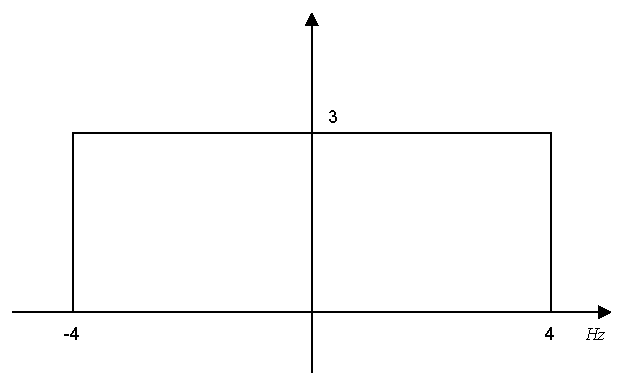
\includegraphics[width=.8\textwidth]{img/fig_1.pdf}
		\caption*{Rappresentazione grafica del segnale $F\left(\mu\right)$.}
	\end{figure}

	\noindent
	Poi si costruisce il segnale da rimuovere. Quindi, una box con sopra un triangolo:
	\begin{equation*}
		G\left(\mu\right) = \Pi\left(\dfrac{\mu}{2}\right) + \Lambda\left(\dfrac{\mu}{1}\right)
	\end{equation*}
	\begin{figure}[!hpt]
		\centering
		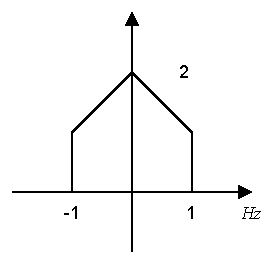
\includegraphics[width=.45\textwidth]{img/fig_2.pdf}
		\caption*{Rappresentazione grafica del segnale $G\left(\mu\right)$.}
	\end{figure}\newpage

	\noindent
	Infine, si rimuove il segnale. Per farlo, si capovolge il segnale $G\left(\mu\right)$ e poi si somma al segnale $F\left(\mu\right)$:
	\begin{equation*}
		L\left(\mu\right) = F\left(\mu\right) - G\left(\mu\right) = 3\Pi\left(\dfrac{\mu}{8}\right) - \Pi\left(\dfrac{\mu}{2}\right) - \Lambda\left(\dfrac{\mu}{1}\right)
	\end{equation*}
	\begin{figure}[!hpt]
		\centering
		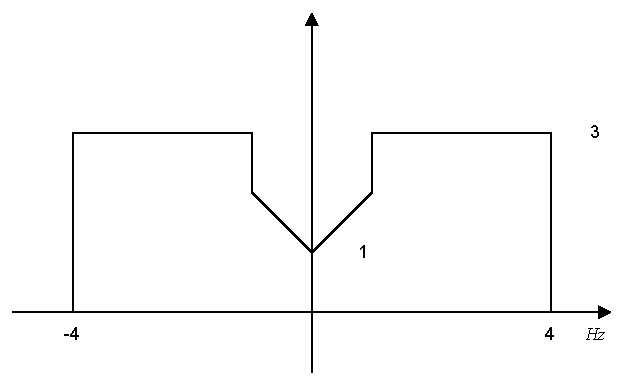
\includegraphics[width=\textwidth]{img/fig_3.pdf}
		\caption*{Rappresentazione grafica del segnale $L\left(\mu\right)$.}
	\end{figure}
	
	\noindent
	Per creare i due trapezoidi, è necessario fare una convoluzione tra due box. Successivamente, si esegue la convoluzione con due impulsi unitari così da shiftare i segnali. I due box devono essere di larghezza $2$ e $4$, così che la lunghezza del trapezoide sia di $6$. Inoltre, per avere un'ampiezza pari a $1$ è necessario avere una box alta $1$ e l'altra di $0.5$ poiché la moltiplicazione delle due ampiezze per la larghezza più piccolo (in questo caso 2), consente di ottenere $1$. L'algoritmo utilizzato per determinare questa convoluzione è derivato da questo \href{https://youtu.be/nHahox9pCg0}{video} e dalla teoria della convoluzione ovviamente.\newline
	
	\noindent
	Quindi, si creano le due box:
	\begin{equation*}
		\begin{array}{lll}
			A\left(\mu\right) & = & \Pi\left(\dfrac{\mu}{2}\right) \\
			\\
			B\left(\mu\right) & = & \dfrac{1}{2}\Pi\left(\dfrac{\mu}{4}\right)
		\end{array}
	\end{equation*}\newpage

	\begin{figure}[!htp]
		\centering
		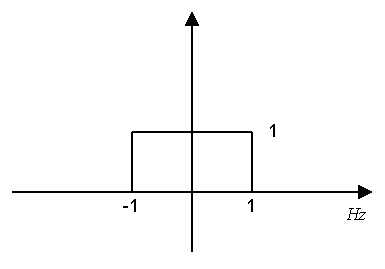
\includegraphics[width=.4\textwidth]{img/fig_4.pdf}
		\caption*{Rappresentazione grafica del segnale $A\left(\mu\right)$.}
	\end{figure}
	
	\begin{figure}[!htp]
		\centering
		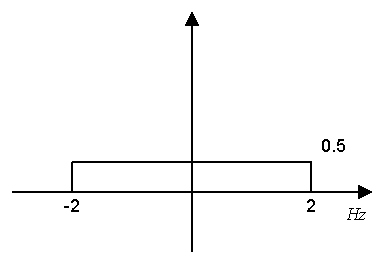
\includegraphics[width=.4\textwidth]{img/fig_5.pdf}
		\caption*{Rappresentazione grafica del segnale $B\left(\mu\right)$.}
	\end{figure}
	
	\noindent
	Adesso si effettua la convoluzione dei due segnali così da ottenere un romboide e successivamente si esegue due convoluzioni distinte: una con un impulso shiftato nella parte dei positivi e una sempre con un impulso shiftato nella parte dei negativi.
	\begin{equation*}
		C\left(\mu\right) = \left[A\left(\mu\right) * B\left(\mu\right)\right] * \left[\delta\left(\mu - 7\right) + \delta\left(\mu + 7\right)\right] =
		\left[\Pi\left(\dfrac{\mu}{2}\right) * \dfrac{1}{2}\Pi\left(\dfrac{\mu}{4}\right)\right] * \left[\delta\left(\mu - 7\right) + \delta\left(\mu + 7\right)\right]
	\end{equation*}
	\begin{figure}[!htp]
		\centering
		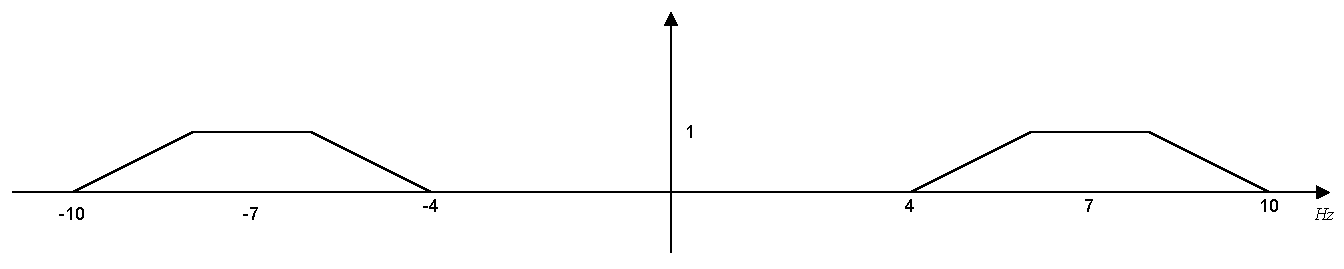
\includegraphics[width=\textwidth]{img/fig_6.pdf}
		\caption*{Rappresentazione grafica del segnale $C\left(\mu\right)$.}
	\end{figure}\newpage
	
	\noindent
	Quindi il grafico finale avrà la seguente forma analitica:
	\begin{equation*}
		R\left(\mu\right) = L\left(\mu\right) + C\left(\mu\right) = 3\Pi\left(\dfrac{\mu}{8}\right) - \Pi\left(\dfrac{\mu}{2}\right) - \Lambda\left(\dfrac{\mu}{1}\right) + \left[\Pi\left(\dfrac{\mu}{2}\right) * \dfrac{1}{2}\Pi\left(\dfrac{\mu}{4}\right)\right] * \left[\delta\left(\mu - 7\right) + \delta\left(\mu + 7\right)\right]
	\end{equation*}
	
	\begin{figure}[!htp]
		\centering
		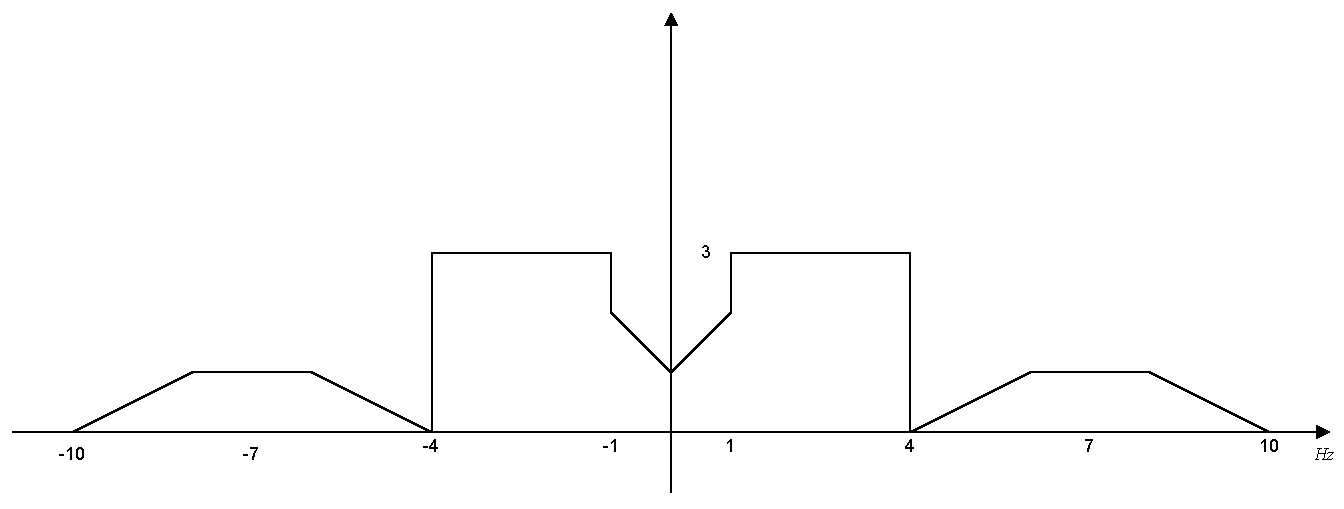
\includegraphics[width=\textwidth]{img/fig_7.pdf}
		\caption*{Rappresentazione grafica del segnale finale.}
	\end{figure}\newpage

	\section{Soluzione Esercizio (5 punti)}
	
	La funzione segno $\mathrm{sgn}$ è definita nel seguente modo:
	\begin{equation*}
		\mathrm{sgn}\left(x\right) = \begin{cases}
			+1 & x>0 \\
			-1 & x<0 \\
			0  & x=0
		\end{cases}
	\end{equation*}
	Dato il segnale:
	\begin{equation*}
		s\left(t\right) = \mathrm{sgn}\left(a \cdot \cos\left(\dfrac{2\pi}{T_{0}}t\right)\right)
	\end{equation*}
	Per rappresentarlo graficamente è necessario dare un certo periodo. Per esempio, si prenda il valore $6$:
	\begin{figure}[!htp]
		\centering
		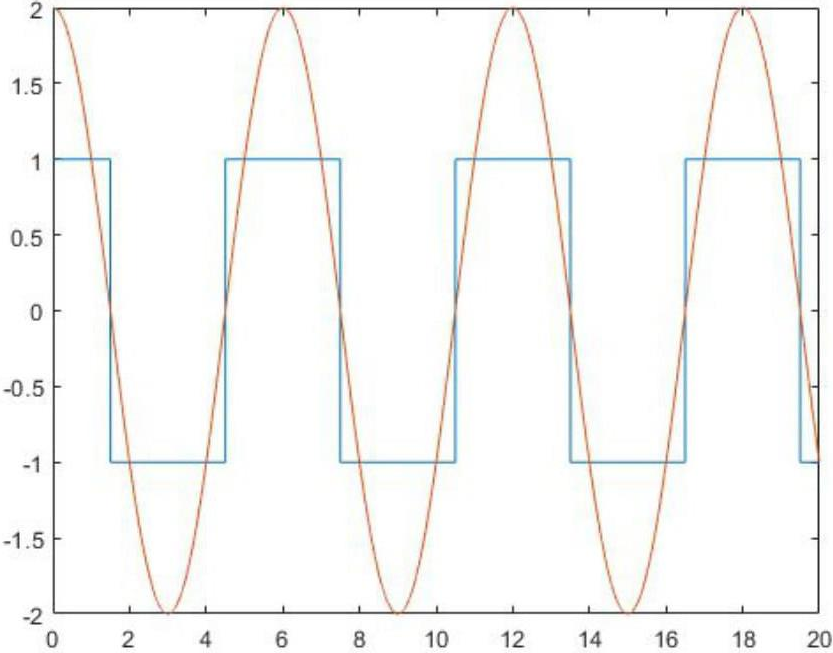
\includegraphics[width=.8\textwidth]{img/fig_8.png}
	\end{figure}
	
	\noindent
	L'energia di un segnale è definita nel seguente modo:
	\begin{equation*}
		E_{f} = \begin{cases}
			\displaystyle\int_{-\infty}^{+\infty} f^{2}\left(t\right) \mathrm{d}t & \text{se }f \in \mathbb{R} \\
			\\
			\displaystyle\int_{-\infty}^{+\infty} \left|f\left(t\right)\right|^{2} \mathrm{d}t \hspace{2em} \text{con } \left|f\left(t\right)\right|^{2} = \tilde{f}\left(t\right)f\left(t\right) & \text{se }f \in \mathbb{C}
		\end{cases}
	\end{equation*}
	E la sua unità di misura è il \emph{joule}.\newpage

	\noindent
	Quindi, dato che la funzione $\cos$, pensando alla forma di Eulero, è appartenente al dominio dei complessi, si sceglie il secondo integrale:
	\begin{equation*}
		E_{s} = \displaystyle\int_{-\infty}^{+\infty} \left|s\left(t\right)\right|^{2} \mathrm{d}t =
		\displaystyle\int_{-\infty}^{+\infty} \left| \mathrm{sgn}\left(a \cdot \cos\left(\dfrac{2\pi}{T_{0}}t\right)\right) \right|^{2} \mathrm{d}t =
		\displaystyle\int_{-\infty}^{+\infty} 1 \:\mathrm{d}t
	\end{equation*}
	Data la definizione della funzione segno, essa ritorna sempre $1$ o $-1$ con un valore diverso da zero. Per cui, dato che il coseno nella peggiore delle ipotesi può essere $1$ (con $\cos\left(0\right) = 1$), se $a$ è sempre diverso da zero, il risultato ottenuto dalla funzione segno e elevato alla seconda sarà sempre positivo e pari a uno. Svolgendo l'integrale si ha dunque:
	\begin{equation*}
		\left[s\right]_{-\infty}^{+\infty} = +\infty+\infty = +\infty
	\end{equation*}
	Risulta evidente che il segnale non ha energia finita poiché per esserlo il risultato deve essere un numero finito. Tuttavia, è possibile affermare che il segnale sia un segnale d'energia.\newline
	
	\noindent
	La potenza media di un segnale è definita nel seguente modo:
	\begin{equation*}
		P_{f} = \begin{cases}
			\displaystyle\lim_{T\rightarrow\infty} \dfrac{1}{T} \displaystyle\int_{-\frac{T}{2}}^{+\frac{T}{2}} f^{2}\left(t\right)\mathrm{d}t & \text{se } f \in \mathbb{R} \\
			\\
			\displaystyle\lim_{T\rightarrow\infty} \dfrac{1}{T} \displaystyle\int_{-\frac{T}{2}}^{+\frac{T}{2}} \left|f\left(t\right)\right|^{2}\mathrm{d}t \hspace{2em} \text{con } \left|f\left(t\right)\right|^{2} = \tilde{f}\left(t\right)f\left(t\right) & \text{se } f \in \mathbb{C}
		\end{cases}
	\end{equation*}
	L'unità di misura è il \emph{watt}.	Analogo all'integrale dell'energia si ha lo stesso risultato:
	\begin{equation*}
		P_{s} = \displaystyle\lim_{T\rightarrow\infty} \dfrac{1}{T} \displaystyle\int_{-\frac{T}{2}}^{+\frac{T}{2}} \left|s\left(t\right)\right|^{2}\mathrm{d}t = 
		\displaystyle\lim_{T\rightarrow\infty} \dfrac{1}{T} \displaystyle\int_{-\frac{T}{2}}^{+\frac{T}{2}} \left| \mathrm{sgn}\left(a \cdot \cos\left(\dfrac{2\pi}{T_{0}}t\right)\right) \right|^{2}\mathrm{d}t = \displaystyle\int_{-\frac{T}{2}}^{\frac{T}{2}} 1 \:\mathrm{d}t
	\end{equation*}
	Il risultato è di nuovo banale e si sostituiscono gli estremi dell'integrale:
	\begin{equation*}
		\displaystyle\lim_{T \rightarrow \infty} \dfrac{1}{T}\left[x\right]_{-\frac{T}{2}}^{+\frac{T}{2}} =
		\displaystyle\lim_{T \rightarrow \infty} \dfrac{\dfrac{T}{2} + \dfrac{T}{2}}{T} = 1
	\end{equation*}
	La potenzia media è $1$, di conseguenza l'integrale converge e il segnale ha una potenza finita.\newpage
	
	\section{Soluzione Esercizio (5 punti)}
	
	L'operazione di equalizzazione di un'immagine è un calcolo piuttosto semplice.\newline
	
	\noindent
	Il \textbf{primo passo} è numerare i livelli di grigio presenti all'interno dell'immagine. L'insieme dei livelli di grigio sarà denotato con la lettera $r_{k}$ e con la lettera $k$ si indicherà il $k$-esimo livello di grigio. Quindi, si riporta per comodità la matrice e si elencano i livelli di grigio:
	\begin{table}[!htbp]
		\centering
		\begin{tabular}{@{} c | c | c @{}}
			\toprule
			3 & 1 & 1 \\
			1 & 7 & 6 \\
			0 & 2 & 1 \\
			\bottomrule
		\end{tabular}
	\end{table}
	\begin{equation*}
		r_{k} = \left\{0, 1, 2, 3, 4, 5, 6, 7\right\} \hspace{2em} \text{con } r_{1} = 0, r_{2} = 1, ..., r_{8} = 7
	\end{equation*}
	In altre parole, l'insieme indica tutti i possibili valori che ci sono all'interno della matrice in ordine crescente.\newline
	
	\noindent
	Il \textbf{secondo passo} è contare le occorrenze di ogni elemento di $r_{k}$. L'insieme delle occorrenze sarà indicato con $H\left(r_{k}\right)$:
	\begin{equation*}
		\begin{array}{rlllllllll}
			r_{k} 				& = & 0,& 1,& 2,& 3,& 4,& 5,& 6,& 7 \\
			\\
			H\left(r_{k}\right) & = & 1,& 4,& 1,& 1,& 0,& 0,& 1,& 1
		\end{array}
	\end{equation*}
	Quindi, lo zero si ripete $1$ volta all'interno della matrice, l'uno si ripete $4$ volte, il due si ripete una volta e così via fino al valore $7$ che si ripete $1$ volta.\newline
	
	\noindent
	Il \textbf{terzo passo} è applicare la seguente formula, che rappresenta una sorta di probabilità:
	\begin{equation*}
		p_{r}\left(r_{k}\right) = \dfrac{H\left(r_{k}\right)}{M \cdot N}
	\end{equation*}
	In cui $M,N$ sono il numero di righe e colonne della matrice, quindi $3 \times 3 = 9$. Si applica a ciascun elemento dell'insieme $r_{k}$:
	\begin{equation*}
		\begin{array}{rccccccccc}
			r_{k} 					& = & 0,& 1,& 2,& 3,& 4,& 5,& 6,& 7 \\
			\\
			H\left(r_{k}\right) 	& = & 1,& 4,& 1,& 1,& 0,& 0,& 1,& 1 \\
			\\
			p_{r}\left(r_{k}\right) & = & \dfrac{1}{9},& \dfrac{4}{9},& \dfrac{1}{9},& \dfrac{1}{9},& \dfrac{0}{9},& \dfrac{0}{9},& \dfrac{1}{9},& \dfrac{1}{9}
		\end{array}
	\end{equation*}\newpage
	
	\noindent
	Il \textbf{quarto passo} è la normalizzazione, indicata con $S$ dei valori. Essa è una somma cumulativa dei valori $p_{r}\left(r_{k}\right)$ e ciascun valore, della somma, si moltiplica per il valore massimo di grigio (in questo caso $7$):
	\begin{equation*}
		\begin{array}{rccccccccc}
			r_{k} 						& = & 0,& 1,& 2,& 3,& 4,& 5,& 6,& 7 \\
			\\
			H\left(r_{k}\right) 		& = & 1,& 4,& 1,& 1,& 0,& 0,& 1,& 1 \\
			\\
			p_{r}\left(r_{k}\right) 	& = & \dfrac{1}{9},& \dfrac{4}{9},& \dfrac{1}{9},& \dfrac{1}{9},& \dfrac{0}{9},& \dfrac{0}{9},& \dfrac{1}{9},& \dfrac{1}{9} \\
			\\
			\sum p_{r}\left(r_{k}\right)& = & \dfrac{1}{9},& \dfrac{5}{9},& \dfrac{6}{9},& \dfrac{7}{9},& \dfrac{7}{9},& \dfrac{7}{9},& \dfrac{8}{9},& \dfrac{9}{9}
		\end{array}
	\end{equation*}
	Adesso che è stata esplicitata la somma cumulativa, si moltiplica ogni frazione per il valore massimo di grigio ($7$) e poi si esegue un arrotondamento per eccesso da $0.5$ a $0.9$, altrimenti per difetto:
	\begin{equation*}
		\begin{array}{lllllll}
			r_{k} = 0 & \longrightarrow & \dfrac{1}{9} \cdot 7 & = & 0.777 & \longrightarrow & 1 \\
			\\
			r_{k} = 1 & \longrightarrow & \dfrac{5}{9} \cdot 7 & = & 3.885 & \longrightarrow & 4 \\
			\\
			r_{k} = 2 & \longrightarrow & \dfrac{6}{9} \cdot 7 & = & 4.662 & \longrightarrow & 5 \\
			\\
			r_{k} = 3 & \longrightarrow & \dfrac{7}{9} \cdot 7 & = & 5.439 & \longrightarrow & 5 \\
			\\
			r_{k} = 4 & \longrightarrow & \dfrac{7}{9} \cdot 7 & = & 5.439 & \longrightarrow & 5 \\
			\\
			r_{k} = 5 & \longrightarrow & \dfrac{7}{9} \cdot 7 & = & 5.439 & \longrightarrow & 5 \\
			\\
			r_{k} = 6 & \longrightarrow & \dfrac{8}{9} \cdot 7 & = & 6.216 & \longrightarrow & 6 \\
			\\
			r_{k} = 7 & \longrightarrow & \dfrac{9}{9} \cdot 7 & = & 7 & \longrightarrow & 7
		\end{array}
	\end{equation*}\newline
	
	\noindent
	Il \textbf{quinto e ultimo passo} è riscrivere la matrice equalizzata andando a sostituire i valori $r_{k}$ con la rispettiva normalizzazione (quindo gli zero con $1$, gli uni con $4$, e così via):
	\begin{table}[!htbp]
		\centering
		\begin{tabular}{@{} c | c | c @{}}
			\toprule
			5 & 4 & 4 \\
			4 & 7 & 6 \\
			1 & 5 & 4 \\
			\bottomrule
		\end{tabular}
	\end{table}
\end{document}